%!TEX root = ..\main.tex
\section{Langevin Dynamics}
\label{sec:langevin_dynamics}

\subsection{Langevin equations}
\label{subsec:langevin_equations}
To study dynamics we ran Langevin dynamics simulations. Accordingly, each particle trajectory is obtained by solving two stochastic differential equations,
\begin{equation}
\label{eq:langevin_theory_1}
	\dot{\boldsymbol{r}}(t) = \boldsymbol{v}(t)
\end{equation}
and
\begin{equation}
\label{eq:langevin_theory_2}
	m \dot{\boldsymbol{v}}(t) = \boldsymbol{f}(\boldsymbol{r}, t) - \alpha_{tr} \boldsymbol{v}(t) + \boldsymbol{\beta}_{tr}(t)
	,
\end{equation}
where $m$ is the particle mass, $\boldsymbol{r}$ and $\boldsymbol{v}$ are the particle coordinates and velocity,  $\alpha_{tr}$ is the damping coefficient related to the drag \textcolor{red}{I think it's rather relevant that its drag from surrounding medium and not other particles, or its just obvious?}, and $f(r, t)$ is a force acting on a particle, which comprises of interparticular interaction and external forces \textcolor{red}{like some external potential, which we currently do not have}. $\boldsymbol{\beta}_{tr}$ is a stochastic force, and in order to satisfy dissipation-fluctuation theorem, every component of it is assumed to be Gaussian-distributed, with
\begin{equation}
\langle\beta_{tr}(t)\rangle = 0
\end{equation}
and
\begin{equation}
\label{eq:stochastic_term_dispersion}
	\langle\beta_{tr}(t)\beta_{tr}(t')\rangle = 2 \alpha_{tr} k_B 		T\delta(t - t')
	,
\end{equation}
where $k_B$ is the Boltzmann constant, $T$ is thermostat temperature, $\delta$ is the Dirac delta function and the average is an ensemble average.

The trajectory of rotation motion is obtained by solving two stochastic differential equations,
\begin{equation}
\label{eq:langevin_theory_3}
	\dot{\boldsymbol{\phi}}(t) = \boldsymbol{\omega}(t)
\end{equation}
and
\begin{equation}
\label{eq:langevin_theory_4}
	m \dot{\boldsymbol{\omega}}(t) = \boldsymbol{\tau}(r, t) - \alpha_{r} \boldsymbol{\omega}(t) + \boldsymbol{\beta}_{r}(t)
	,
\end{equation}
where $\phi$ is particle orientation angles, $\omega$ is the angular velocity, $I$ is the inertia and $\tau$ is the torque exerted on a particle \textcolor{red}{By other particles or external field alike}. $\boldsymbol{\beta}_{r}(t)$ is the torque resulting from stochastic force rotating particle, and its components are also assumed to be Gaussian-distributed with zero mean

As we can see from Eqs.~(\ref{eq:langevin_theory_1}, \ref{eq:langevin_theory_2}, \ref{eq:langevin_theory_3}, \ref{eq:langevin_theory_4}), for the rotational motion the form of equations remains unchanged, and they are equivalent to the translation equations under following transformation.
\begin{equation}
\label{eq:rotation_translation_substitution}
	\begin{aligned}[c]
		\boldsymbol{\phi} &\rightarrow \boldsymbol{r}        \\
		\boldsymbol{\omega} &\rightarrow \boldsymbol{v} 
	\end{aligned}
	\qquad
	\qquad
	\begin{aligned}[c]
		I &\rightarrow m        \\
		\boldsymbol{\tau}(r, t) &\rightarrow \boldsymbol{f}(r, t)
	\end{aligned}
\end{equation}

The scalar values are transformed as is, while vectors are replaced with pseudo-vectors.

The damping coefficients $\alpha$ for translation ($\alpha_{tr}$) and rotation ($\alpha_r$) are different, and can be obtained in following way.

First to simplify the particle-medium interaction we need to define damping time $\tau$, which determines how rapidly thermal fluctuations in particles positions and orientations decays, and for translational motion it is given by
\begin{equation}
\label{eq:Translation_damping_time}
	\tau_{tr} = \frac{m}{6 \pi \eta R}
	,
\end{equation}
where $m$ is the particle mass, $\eta$ is the viscosity and $R$ is the particle radius. For rotation $\tau_{tr} / \tau_{r} = 10/3$, which can be obtained from Stokes-Einstein-Debye relations and relation between particle mass and inertia.

And then the $\alpha_t$ and $\alpha_r$ are defined
\begin{equation}
	\begin{aligned}
		\alpha_{tr} = \frac{m}{\tau_{tr}}
	\end{aligned}
	\qquad
	\qquad
	\begin{aligned}
		\alpha_r = \frac{I}{\tau_r}
	\end{aligned}
	,
\end{equation}
where $m$ is the particle mass, $I$ is the inertia, $\tau_{tr,r}$ are the damping times.

\subsection{Integration method}
\label{subsec:integration_method}

The integration scheme for translational equations of motion proposed in~\cite{Taylor2013} is as follows
\begin{equation}
\label{eq:tr_coordinate_change}
	\boldsymbol{r}^{n+1} = \boldsymbol{r}^n + dt \left(
	 b_{tr} \boldsymbol{v}^n
	 + \frac{b_{tr} dt}{2m}\boldsymbol{f}^n
	 + \frac{b_{tr}}{2m}\boldsymbol{\beta}_{tr}^{n+1}
	\right)
\end{equation}
\begin{equation}
\label{eq:tr_velocity_change}
	\boldsymbol{v}^{n+1} = \boldsymbol{v}^n 
	 + \frac{dt}{2m}\left(
	 	\boldsymbol{f}^n + \boldsymbol{f}^{n+1}
	 \right)
	 - \frac{\alpha_{t}}{m}\left(
	 	\boldsymbol{r}^{n+1} - \boldsymbol{r}^n
	 \right)
	 + \frac{1}{m}\boldsymbol{\beta}_{tr}^{n+1}
	 .
\end{equation}
In the above equations, the $dt$ is integration time step, the $n$ index is time steps, $b_{tr}$ accounts for the drag, and $\boldsymbol{\beta}_{tr}^{n+1}$ is a stochastic force at the time $n+1$. Important to note that we use the same stochastic force for coordinates and velocity calculations, which reduces computation time. $\boldsymbol{f}^n$ is the force acting on the particle at the time $n$.
\textcolor{red}{the $ _{tr}$ index is for the translation, it's now consistent with what was above. Do I need to specifically state it? The index $ ^{n+1}$ in the random term due to that at $n=0$ there is no random force. Anyway, as long as it's only one random force it's all the same - they are all uncorrelated}

The same integration scheme can be used for rotation, with proper change of variables (see Eq.~(\ref{eq:rotation_translation_substitution}))
\begin{equation}
\label{eq:rot_angle_change}
	\boldsymbol{\phi}^{n+1} = \boldsymbol{\phi}^n + dt \left(
		  b_{r} \boldsymbol{\omega}^n
		  + \frac{b_{r} dt}{2I}\boldsymbol{\tau}^n
		  + \frac{b_{r} }{2I}\boldsymbol{\beta}_{r}^{n+1}
	 \right)
\end{equation}
\begin{equation}
\label{eq:rot_ang_velocity_change}
	\boldsymbol{\omega}^{n+1} = \boldsymbol{\omega}^n
	+ \frac{dt}{2m}\left(
		\boldsymbol{\tau}^n + \boldsymbol{\tau}^{n+1}
	\right)
	- \frac{\alpha_{r}}{I}\Delta \boldsymbol{u}
	+ \frac{1}{I}\boldsymbol{\beta}_{r}^{n+1}
\end{equation}
here $\Delta \boldsymbol{u} \equiv \left(\boldsymbol{\phi}^{n+1} - \boldsymbol{\phi}^n\right)$ is rotation of the particle within one integration step. Vector $\Delta u$ is parallel to the axis around which particle has rotated on the angle $|\Delta u|$ radians. The coefficients $b_{tr}$ and $b_{r}$ account for the drag exerted on a particle by surrounding medium,
\begin{equation}
\label{eq:drag_coefficient}
	\begin{aligned}
		b_{tr} = \frac{1}{1 + \frac{\alpha_{tr} dt}{2 m}}
	\end{aligned}
	\qquad
	\text{and}
	\qquad
	\begin{aligned}
		b_r = \frac{1}{1 + \frac{\alpha_r dt}{2 I}}
	\end{aligned}
	.
\end{equation}
\textcolor{red}{I think I'm doing it wrong, but that period mark after the equation is really confusing}

When $\alpha_{tr} = 0$, from Eq.~\eqref{eq:drag_coefficient}, we obtain $b_{tr} = 1$ and from Eq.~\eqref{eq:stochastic_term_dispersion} we obtain $\langle\beta_{tr}(t)\beta_{tr}(t')\rangle = 0$. Then the above equations reduces to the standard velocity-Verlet scheme. The damping is calculated as integral  over real path travelled by particle within time step (under assumption that damping time does not change within $dt$ and $\Delta r$) \textcolor{red}{Yes, the damping time is constant, but if it isn't, this assumption is enough for this scheme to work. I never said that it isn't a constant}.

If using integration scheme defined in Eq.~(\ref{eq:rot_angle_change}), effective angular velocity of a particle within every time step is
\begin{equation}
\label{eq:effective_angular_velocity}
	\tilde{\boldsymbol{\omega}}^n = b_{r} \boldsymbol{\omega}^n
	+ \frac{b_{r} dt}{2I}\boldsymbol{\tau}^n
	+ \frac{b_{r} }{2I}\boldsymbol{\beta}_{r}^{n+1}.
\end{equation}

By the definition, angular velocity $\tilde{\omega}^n$ is directed parallel to the axis around which particle is rotated by an angle of $|\tilde{\omega}^n|dt$ per time step $dt$. Therefore, if particle orientation is defined by quaternion $q$, then Eq.~\eqref{eq:rot_angle_change} can be written as
\begin{equation}
q^{n+1} = \tilde{q}\,^n q^{n} ,
\end{equation}
where $q^n$ and $q^{n+1}$ is the quaternion representation of orientation on time steps $n$ and $n+1$ respectively, and $\tilde{q}\,^n q^{n}$ is quaternion multiplication. $\tilde{q}\,^n$ is the quaternion representation of rotation around $\tilde{\omega}^n$ by the angle $|\tilde{\omega}^n|$.

\subsection{Interactions}

To perform simulations we need to define forces acting on the particles.

First of all, as in the Monte-Carlo simulations we restrict interactions to the immediate neighbors (particle $i$ interacts only with particles $i+1$ and $i-1$).

The force acting on a particle is defined by gradient of potential energy.
\begin{equation}
\label{eq:full_force}
	\boldsymbol{F}_{ij}
		= -\boldsymbol{\nabla} E_{ij}
		=  \frac{\hat{r}}{r^4} \left[3 D - A\, r^2 (k r +1) \, \exp(-k r) \right],
\end{equation}
where $D = 3 \cos \theta_1 \cos \theta_2 - (\hat{m}_1 \cdot \hat{m}_2)$ stands for orientational part of dipole-dipole potential and $\boldsymbol{r}$ connects particle centers. The other parameters are the same as in Eqs.~\eqref{eq:dipole_dipole_1D}~and~\eqref{eq:yukawa_interaction}.

The torque on a particle results only from the dipole-dipole interaction. Therefore it is calculated as
\begin{equation}
\label{eq:dipole_torque}
	\boldsymbol{\tau}  = \mu[\hat{\mu} \times \boldsymbol{E}_d ],
\end{equation}
where $\boldsymbol{\mu}$ is dipole moment of particle on which torque acts, and $\boldsymbol{E}_d$ is dipole field produced by acting particle:

\begin{equation}
\label{eq:dipole_field}
	\boldsymbol{E}_d = \frac{\mu}{r^3}
		\left(3 (\hat{\mu} \cdot \hat{r}) \hat{r} - \hat{\mu} \right),
\end{equation}
where $\mu$ is dipole moment of the particle inducing the field.

\subsection{Statistical properties}
For non-interacting spheres the relation between rotational and translational diffusion coefficient can be obtained \cite{C5SM02754C}. The former is given by the Stokes-Einstein relation
\begin{equation}
\label{eq:translational_diffusion_coefficient}
	D_t = \frac{k_B T}{6 \pi \eta R}
\end{equation}
and the latter is given by Stokes-Einstein-Debye relation
\begin{equation}
\label{eq:rotational_diffusion_coefficient}
	D_r = \frac{k_B T}{8 \pi \eta R^3}
	,
\end{equation}
where $T$ is the thermostat temperature, $\eta$ the viscosity of the medium and $k_B$ the Boltzmann constant. The relation between $D_t$ and $D_r$ is given by
\begin{equation}
	\frac{D_r}{D_t} = \frac{3}{4 R^2}
	.
\end{equation}

For sufficiently long times, we can estimate the diffusion coefficient as
\begin{equation}
\label{eq:translation_diffusion_vs_displacement}
	D_t = \lim_{\Delta t \to \infty} \frac{1}{6 \Delta t} \langle r^2(\Delta t)\rangle
	,
\end{equation}
where $\langle r^2(\Delta t)\rangle$ is translational mean square displacement (MSD) of particle relatively to its initial position,
\begin{equation}
	\langle r^2(\Delta t)\rangle
	 = \frac{1}{N} \sum_{i=1}^{N} |\boldsymbol{r}_i(t + \Delta t) - \boldsymbol{r}_i(t)|^2
	 .
\end{equation}

Analogously can be defined relation between rotational diffusion coefficient $D_r$ and rotational mean square displacement (RMSD) $\langle \phi^2(\Delta t) \rangle$
\begin{equation}
\label{eq:rotational_diffusion_vs_displacement}
	D_r = \lim_{\Delta t \to \infty} \frac{1}{6 \Delta t} \langle \phi^2(\Delta t)\rangle
	.
\end{equation}

The vector $\Delta u$ of rotational displacement between two particle orientations represented by quaternions $q^{n+1}$ and $q^n$ can be found in the following way. First, we obtain quaternion $\Delta q = q^{n+1}\, q^{n^{-1}}$, where $q^{n^{-1}}$ is the inverse of $q^n$. Then the direction of $\Delta u$ is parallel to the vector part of $\Delta q$ and $|\Delta u|$ equals to the $\cos^{-1}$ of scalar part of $\Delta q$.

When calculating RMSD we have to account for the fact that rotations on angle $
\alpha$ and $\alpha + 2\pi$ are represented by the same unit quaternions. For that we have to accumulate RD over integration steps (separately for every particle). Then the RMSD can be obtained:

\begin{equation}
\label{eq:rotational_mean_square_displacement}
	\langle \phi^2 (\Delta t)\rangle
		= \frac{1}{N} \sum_{i=1}^{N} 
			\left|
				\sum_{j = 0}^{\frac{\Delta t}{\delta t}}
					\Delta\boldsymbol{u}_{i,j}
			\right|^2
	,
\end{equation}
here we break time interval $\Delta t$ into smaller time intervals $\delta t$, which is necessary due to inability to distinguish rotations on angle $\alpha$ and $\alpha + 2\pi$ radians. The accumulation of rotation goes under summation by $j$ index. \textcolor{red}{The $\Delta t$ could be arbitrary big, so I need to sum the rotation over small intervals where particle turns less then $2 \pi$, or calculate the number of $2 \pi$ rotations. The former is simpler to implement. It's like integrating over path, but splitted into small $\Delta t / \delta t$ pieces, on every one of which we can just use $\Delta u$}

The results of test simulation of non-interacting spheres is shown on \figref{fig:diffusion_stats_mean_square_displacement}. As expected, $\langle r^2\rangle$ is proportional to $2 \cdot \tau_t t$, and $\langle \phi_i^2\rangle$ are proportional to $2 \cdot \tau_r t = 2 \cdot (3/10) \tau_t t$. Here $\tau_t$ is translational damping time defined in eq.~\eqref{eq:Translation_damping_time}, and $t$ is simulation time.

\begin{figure}[h]
\centering
	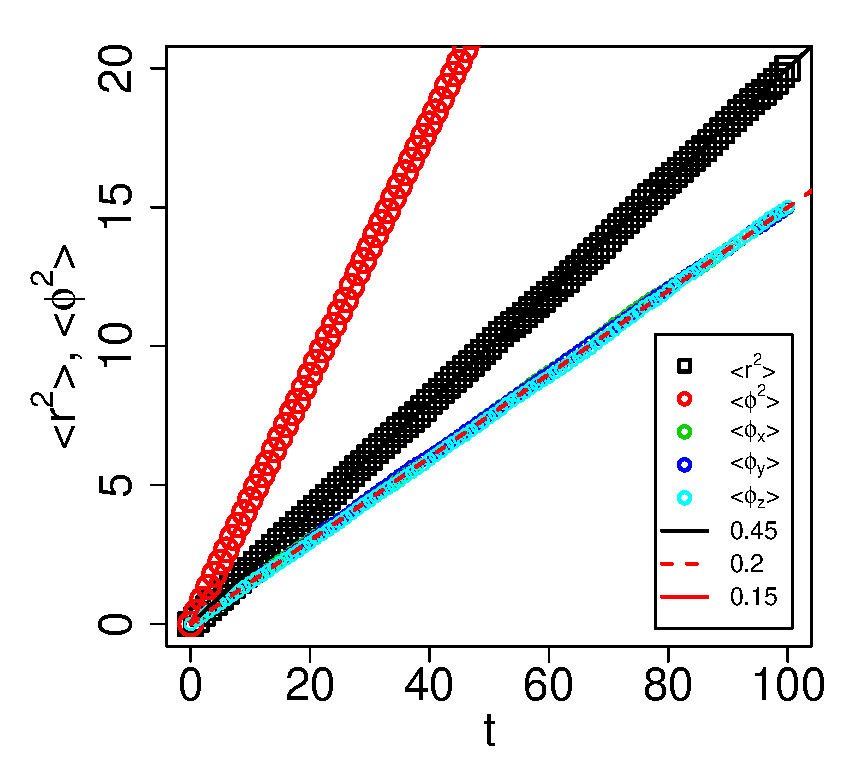
\includegraphics[height=0.3\textheight]{Images/DiffusionStats_drift}
	\captionsetup{justification=centering, width=0.9\textwidth}
	\caption{Particle MSD and RMSD (with components) as function of time. Points are obtained numerically, with averaging over $20000$ samples. Every sample started from $r_z = v_z = \omega_i = 0$ and particle's  dipole moment co-aligned with $z$ axis. Solid lines are theoretical displacement (eqs. \eqref{eq:translation_diffusion_vs_displacement}, \eqref{eq:rotational_diffusion_vs_displacement}) for given $k_BT = 1$, $m = 1$, $R = 1$ and $\tau_t = 0.1$.}
	\label{fig:diffusion_stats_mean_square_displacement}
\end{figure}

Average kinetic energy per degree of freedom is $1/2 \, k_B T$, which for our case of full three-dimensional rotational and one-dimensional translational movement gives $E_k = 2 k_B T$.

At equilibrium, velocity should satisfy Maxwell-Boltzmann distribution
\begin{equation}
\label{eq:maxwell_boltzmann_velocity}
	\begin{aligned}[c]
		p(v^2)
			= \sqrt{ \left(\frac{m}{2 \pi k_B T}\right)^3}
			4 \pi v^2 \exp \left[-\frac{mv_i^2}{2k_BT}\right]
	\end{aligned}
	\qquad
	\begin{aligned}[c]
		p(\omega^2)
			= \sqrt{ \left(\frac{I}{2 \pi k_B T}\right)^3}
			4 \pi \omega^2 \exp\left[-\frac{I\omega_i^2}{2 k_B T}\right]
	\end{aligned}
\end{equation}
where $v$ is translational and $\omega$ is rotational velocity, $m$ is particle mass, and $I$ is particle inertia, $k_B$ is Boltzmann constant and $T$ is thermodynamic temperature.

Velocity components should satisfy normal distribution 
\begin{equation}
\label{eq:maxwell_boltzmann_velocity_components}
	\begin{aligned}[c]
		p(v_i)
			= \sqrt{ \frac{m}{2 \pi k_BT}}
			\exp \left[-\frac{mv_i^2}{2k_BT}\right]
	\end{aligned}
	\qquad
	\begin{aligned}[c]
		p(\omega_i)
			= \sqrt{ \frac{I}{2 \pi k_BT}}
			\exp\left[-\frac{I\omega_i^2}{2k_BT}\right]
	\end{aligned}
\end{equation}

It can be shown that ratio between $\sigma^2_v = k_BT/m$ and $\sigma^2_\omega = k_BT/I$ is
\begin{equation}
\label{eq:velocity_deviation_relation}
	\frac{\sigma^2_v}{\sigma^2_\omega} = \frac{2}{3}R^2
\end{equation}
where $R$ is radius of a particle.

At the \figref{fig:velocity_distributions} the velocity probability distribution are shown, both theoretical and obtained from simulations, for one value of $k_BT = 1$ and $m = 1$. As expected, the $\sigma^2_v / \sigma^2_\omega$ are related as $2/3$ for our case of $R = 1$.

\begin{figure}[h]
\centering
	\begin{subfigure}[t]{0.45\textwidth}
		\centering
		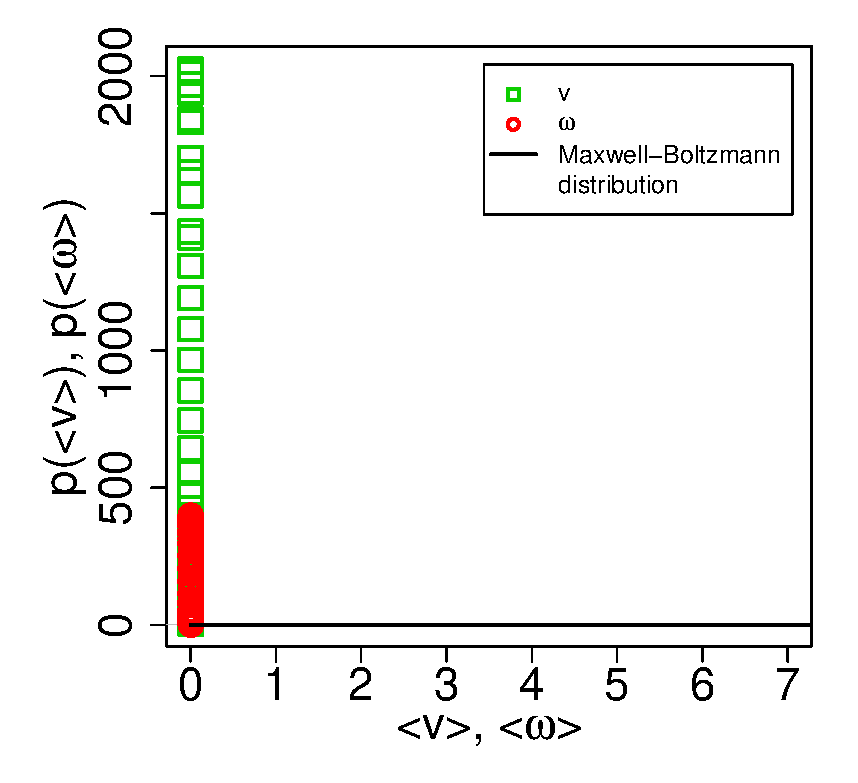
\includegraphics[width=\textwidth]{Images/DiffusionStats_mb}
		\captionsetup{justification=centering, width=0.9\textwidth}
		\caption{Probability distribution of velocity module. Theoretical distribution is given by equation~\eqref{eq:maxwell_boltzmann_velocity}}
	\end{subfigure}
	\begin{subfigure}[t]{0.45\textwidth}
		\centering
		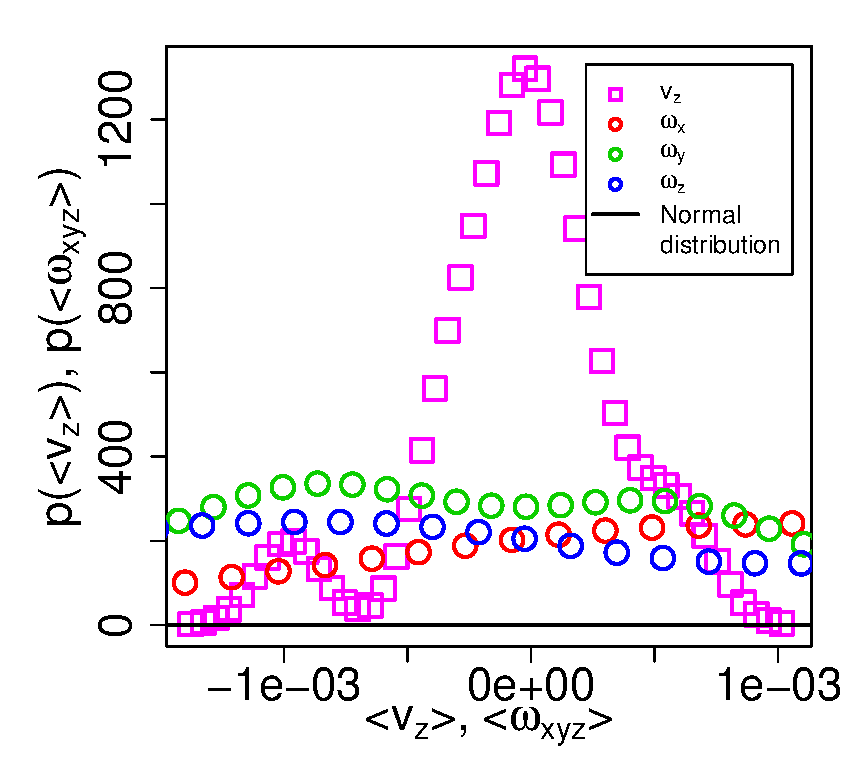
\includegraphics[width=\textwidth]{Images/DiffusionStats_norm}
		\captionsetup{justification=centering, width=0.9\textwidth}
		\caption{Probability distribution of velocity components. Theoretical distribution is given by equation~\eqref{eq:maxwell_boltzmann_velocity_components}}
	\end{subfigure}
	\captionsetup{justification=centering, width=0.9\textwidth}
	\caption{Translational and rotational velocity probability distribution. Points are obtained numerically, with averaging over $20000$ samples. Every sample started from $r_z = v_z = \omega_i = 0$ and particle's dipole moment co-aligned with $z$ axis. Solid lines are theoretical distributions for given $k_BT = 1$ and $m = 1$.}
	\label{fig:velocity_distributions}
\end{figure}